\documentclass{article}
\usepackage[utf8x]{inputenc}
\usepackage{formatting}
\usepackage{multicol}
\usepackage{mathtools}
\usepackage{float}
\usepackage{matlab-prettifier}

\title{Integration in Multiple Dimensions: Answer Key}
\author{Quantitative Engineering Analysis}
\date{\today}

\begin{document}

\maketitle

\section{Review of Single-Variable Calculus}

\paragraph{1.Create a table of five fundamental functions $x^n$, sin(x), cos(x), exp(x), and ln(x). List both their derivatives and their anti-derivatives. Include in your table at least one other example.}


\begin{center}
\begin{tabular}{ |c|c|c|c|c|c| }
\hline
 $nx^{n-1}$ & cos(x) & -sin(x) & $e^x$ & $\dfrac{1}{x}$ & ??? \\ \hline \hline
 $x^n$ & sin(x) & cos(x) & $e^x$ & ln(x) & ???? \\ \hline \hline 
 $\dfrac{x^{n+1}}{n+1}+c$ & -cos(x)+c & sin(x)+c & $e^x+c$ & $xlnx-x+c$ & ????? \\ \hline
\end{tabular}
\end{center}


\paragraph{2.Consider the sketch of the function below. Now try to sketch the derivative and an anti-derivative.}

\begin{figure}[H]
    \centering
    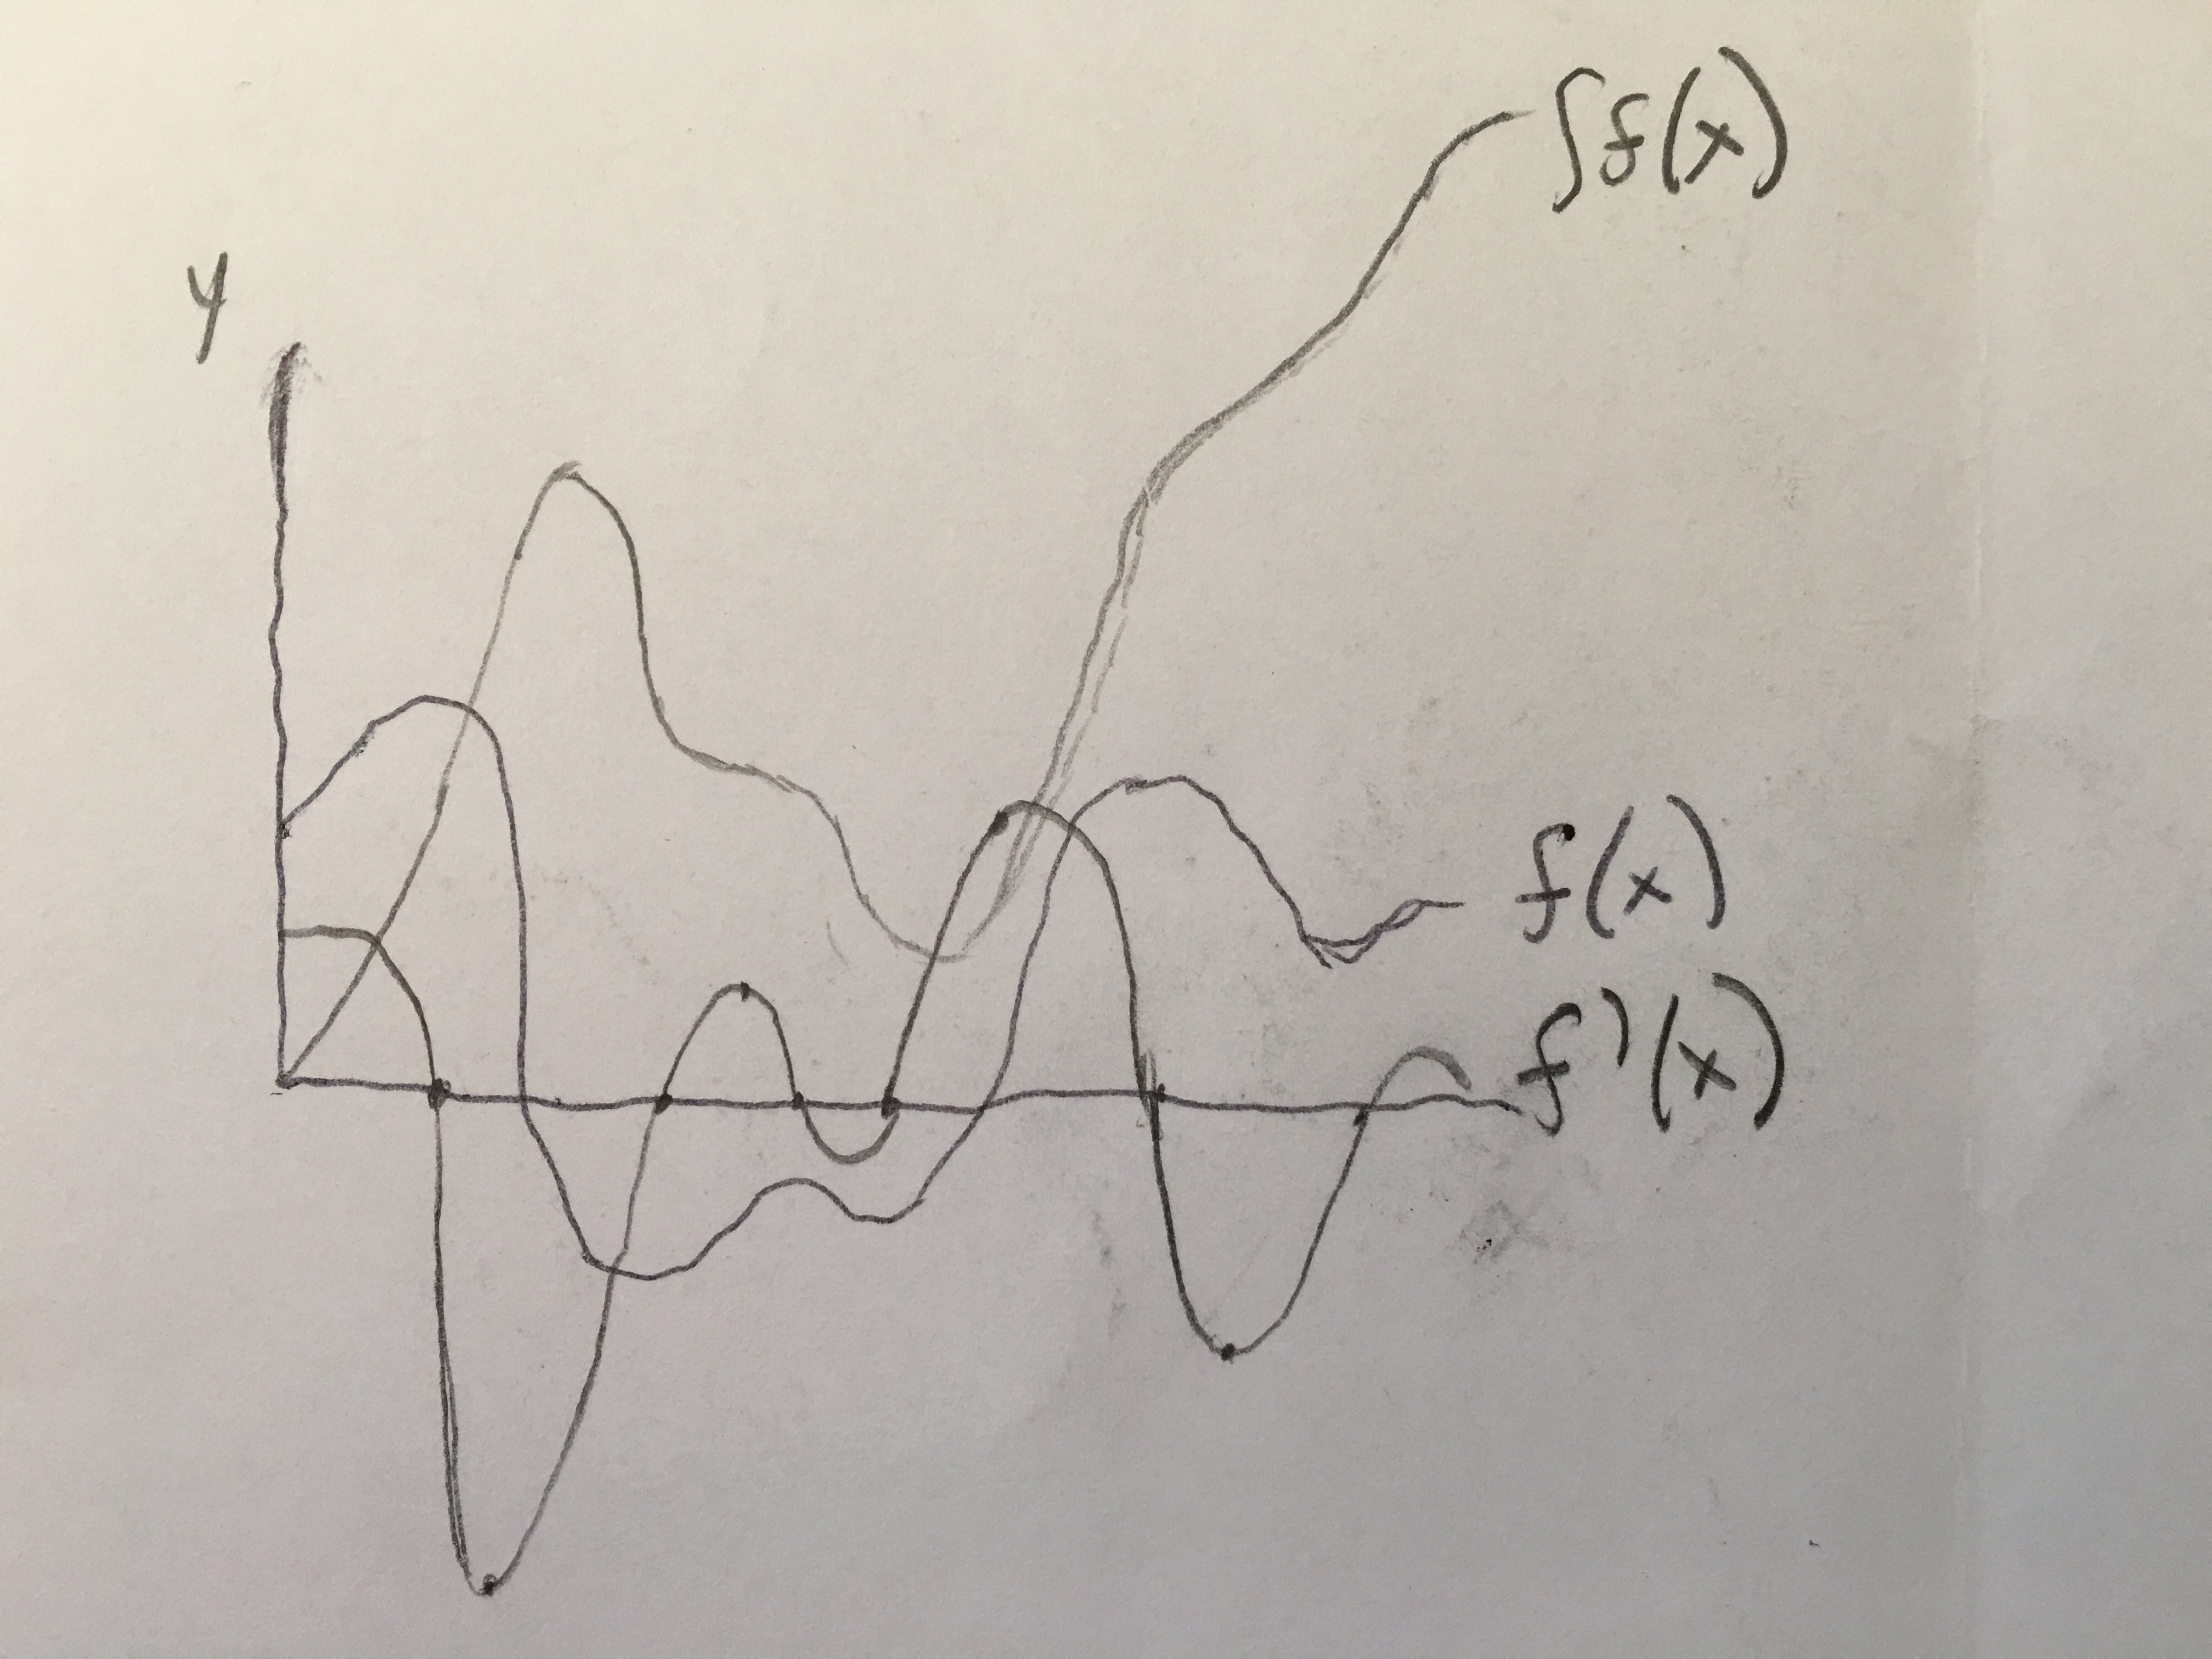
\includegraphics[width=0.5\columnwidth]{sketch.jpg}
    \caption{The derivative and anti-derivative.}
\end{figure}

\paragraph{3. Make a visual argument about why these properties are true.} Below is a visual argument for $(f'+g') = f' + g'$. Students should have some visual representation for each of the four properties.

\begin{figure}[H]
    \centering
    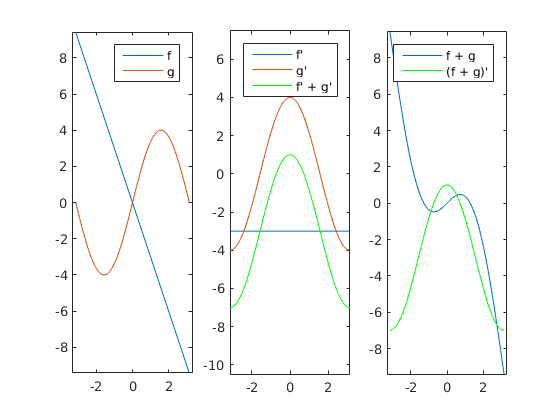
\includegraphics[width=0.5\columnwidth]{visual.png}
    \caption{How cool!}
\end{figure}

\paragraph{4. Use your table of fundamental functions and the chain rule to determine the derivative of $(x^3 − 1)^100$.}

\begin{align*}
    u &= x^3 - 1 \\
    \frac{d}{dx}u^{100} &= \frac{d}{du}u^{100} \frac{du}{dx} \\
    \frac{du}{dx} &= 3x^2 \\
    \frac{d}{du}u^{100} &= 100u^{99} \\
    \frac{d}{dx}(x^3 − 1)^{100} &= 100(x^3 - 1)^{99} (3x^2) \\
    &= 300x^2 (x^3 -1)^{99}
\end{align*}

\paragraph{5. Use your table of fundamental functions and the substitution rule to evaluate $\int_0^4 \sqrt{2x+1}\,dx$}

\begin{align*}
    u &= 2x + 1 \\
    \int u^\frac{1}{2} \, dx &= \int \frac{u^\frac{1}{2} \, du}{\frac{du}{dx}} \\
    &= \frac{1}{2} \int u^\frac{1}{2} \, du \\
    &= \frac{1}{2} \left(\frac{2}{3}u^\frac{3}{2}\right) \\
    &= \frac{1}{3}\left(2x + 1\right)^\frac{3}{2} \\
    &= \frac{26}{3}
\end{align*}

\paragraph{6. Use your table of fundamental functions and the product rule to determine the derivative of $\sqrt{x} (1-x)$.}

\begin{align*}
    &= \sqrt{x} * (-1) + (1 - x) * \left(\frac{1}{2}x^\frac{-1}{2}\right) \\
    &= \frac{-3\sqrt{x}}{2} + \frac{1}{2\sqrt{x}}
\end{align*}

\paragraph{7. Use your table of fundamental functions and integration by parts to determine $\int_1^2 x \exp(-x) \; dx$.}

\begin{align*}
    \int f\,dg &= fg - \int g \, df \\
    f &= x, \; dg = \mathrm{e}^{-x}dx \\
    df &= dx, \; g = -\mathrm{e}^{-x}\\
    fg - \int g \, df &= -x\mathrm{e}^{-x} - \int -\mathrm{e}^{-x} \, dx \\
    &= -\mathrm{e}^{-x}(x + 1) \\
    &= \frac{2\mathrm{e} - 3}{\mathrm{e}^2}
\end{align*}

\paragraph{8. Recall some of the explicit functions you used to describe curves generated by taking sections through fruit, vegetables, or manufactured objects. Propose an integral that would determine the cross-sectional area of the section, and evaluate it.}

\begin{figure}[H]
    \centering
    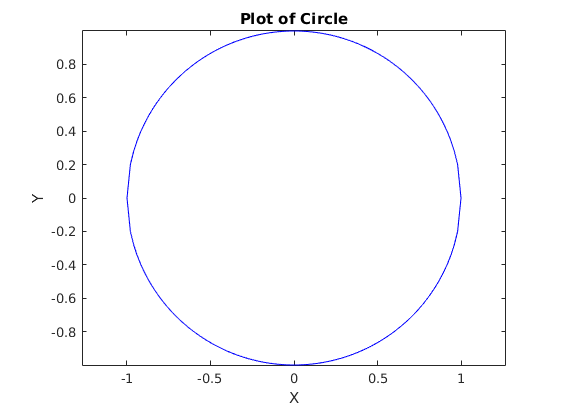
\includegraphics[width=0.5\columnwidth]{circle.png}
    \caption{remember this?}
\end{figure}

\begin{align*}
    \mathrm{Area} &= \int_{-1}^1 \left(\sqrt{1 - x^2} - \left(-\sqrt{1 - x^2}\right)\right) \, dx\\
    &= x\sqrt{1-x^2} + \sin^{-1}x\Bigr|_{-1}^1 \\
    &= \pi
\end{align*}

\paragraph{9. Consider the family of functions defined by the power law, $y = x^n, n = 1,2,3,\ldots$. Propose an integral that would determine the area enclosed on the top by $y=d$, on the bottom by $y = x^n$, on the left by $x=0$, and on the right by the intersection of the top and bottom functions. Evaluate it and graph the enclosed area as a function of the parameter $d$. Use a log-log plot and interpret the result.}

\begin{align*}
    \int_0^{\sqrt[n]{d}} \left(d - x^n \right) \, dx &= x\left(d - \frac{x^n}{n+1}\right) \Bigr|_0^{\sqrt[n]{d}} \\
    &= \sqrt[n]{d}\left(d - \frac{d}{n+1}\right) \\
    &= \sqrt[n]{d}\left(\frac{dn}{n+1}\right)
\end{align*}

\lstinputlisting[style=Matlab-editor,caption=code to graph relationship between d n and area.]{power_law.m}

\begin{figure}[H]
    \centering
    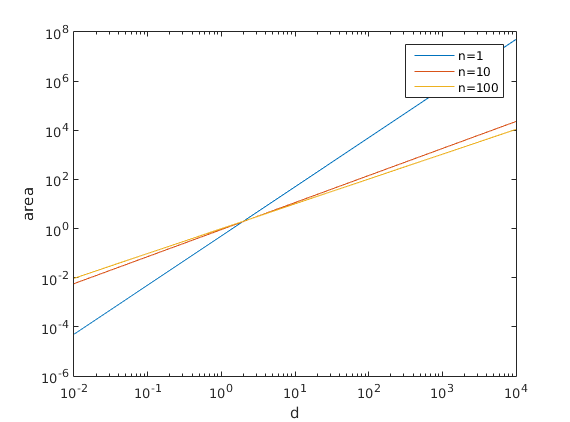
\includegraphics[width=0.75\columnwidth]{power.png}
    \caption{As d increases, the area accumulated increases exponentially. Also, the larger n, the smaller the area accumulated. Try to understand why!}
\end{figure}

\paragraph{10. Evaluate $\frac{\partial f}{\partial x}$ and $\frac{\partial f}{\partial y}$ for $f(x,y) = x^2 \sin(xy^2)$.}

\begin{align*}
   \frac{\partial f}{\partial x} &= x^2 y^2 \cos (x y^2) + 2x\sin(x y^2) \\
   \frac{\partial f}{\partial y} &= 2x^3 y \cos(xy^2)
\end{align*}

\paragraph{11. Evaluate all four second-order derivatives of $f(x,y) = x^2 \sin(xy^2)$.}


\begin{align*}
    \frac{\partial^2 f}{\partial x \partial y} = \frac{\partial^2 f}{\partial y \partial x} &= -2x^2 y\left(xy^2\sin\left(xy^2\right)-3\cos\left(xy^2\right)\right) \\
    \frac{\partial^2 f}{\partial x^2} &= \left(2-x^2y^4\right)\sin(xy^2)+4xy^2\cos(xy^2) \\
    \frac{\partial^2 f}
    {\partial y^2} &= 2x^3 \left(\cos(xy^2)-2xy^2sin(xy^2)\right)
\end{align*}


\paragraph{12. Review the article on partial derivative at {\it http://mathworld.wolfram.com/PartialDerivative.html} Under what conditions on the function $f$ are the mixed partial derivatives equal?}

The function's first derivatives must be differentiable. This can fail if the second partials are not continuous.

\paragraph{13. How many second-order derivatives are there of $f(x,y,z)$?}

12.

\paragraph{14. Sketch the regions of integration and compute the area of the enclosed region by evaluating the double integral.} 
\begin{enumerate}
\item $ \int_0^1 \int_0^x dy dx $

\begin{align*}
    &= \int_{0}^{1}xdx \\
    &= \frac{x^2}{2}\Bigr|_{0}^{1} \\
    &= 1/2
\end{align*}

\item $ \int_0^{\pi/2} \int_0^{\sin x} dy dx $

\begin{align*}
    &= \int_{0}^{\pi/2}\sin xdx \\
    &= -\cos x\Bigr|_{0}^{\pi/2} \\
    &= 1
\end{align*}

\item $ \int_1^2 \int_0^{\ln x} dy dx $

\begin{align*}
    &= \int_{1}^{2}\ln xdx \\
    &= (x\ln x - x)\Bigr|_{1}^{2} \\
    &= 2 \ln2-\ln1-1 = 0.386
\end{align*}

\end{enumerate}

\paragraph{15. Sketch the regions of integration and compute the area of the enclosed region by evaluating the double integral.} 

\begin{enumerate}
\item $ \int_0^1 \int_y^{2-y} dx dy $

\begin{align*}
    &= \int_{1}^{2}2-2y dy \\
    &= 2y-y^2\Bigr|_{0}^{1} \\
    &= 2-1 = 1
\end{align*}

\item $ \int_0^4 \int_{y/2}^2 dx dy $

\begin{align*}
    &= \int_{0}^{4}2-\frac{y}{2} dy \\
    &= 2y-\frac{y^2}{4}\Bigr|_{0}^{4} \\
    &= 8-4 = 4
\end{align*}

\item $ \int_0^1 \int_y^{\exp y} dx dy $

\begin{align*}
    &= \int_{0}^{1}e^y-y dy \\
    &= e^y-\frac{y^2}{2}\Bigr|_{0}^{1} \\
    &= e-\frac{1}{2}-1 = 1.22
\end{align*}

\end{enumerate}

\paragraph{16. Sketch the regions of integration and compute the area of the enclosed region by evaluating the double integral.}

\begin{align*}
    &= \int_{-1}^1 \int_{-1}^{y^2} dxdy + \int_{-1}^1 \int_{1}^{1+x^2} dydx \\
    &= \int_{-1}^1 (y^2 + 1) dy + \int_{-1}^1 x^2 dx
    &= \frac{10}{3}
\end{align*}

\paragraph{17. Sketch the following regions of integration in the plane, and evaluate the double integral.}

\begin{figure}[H]
    \centering
    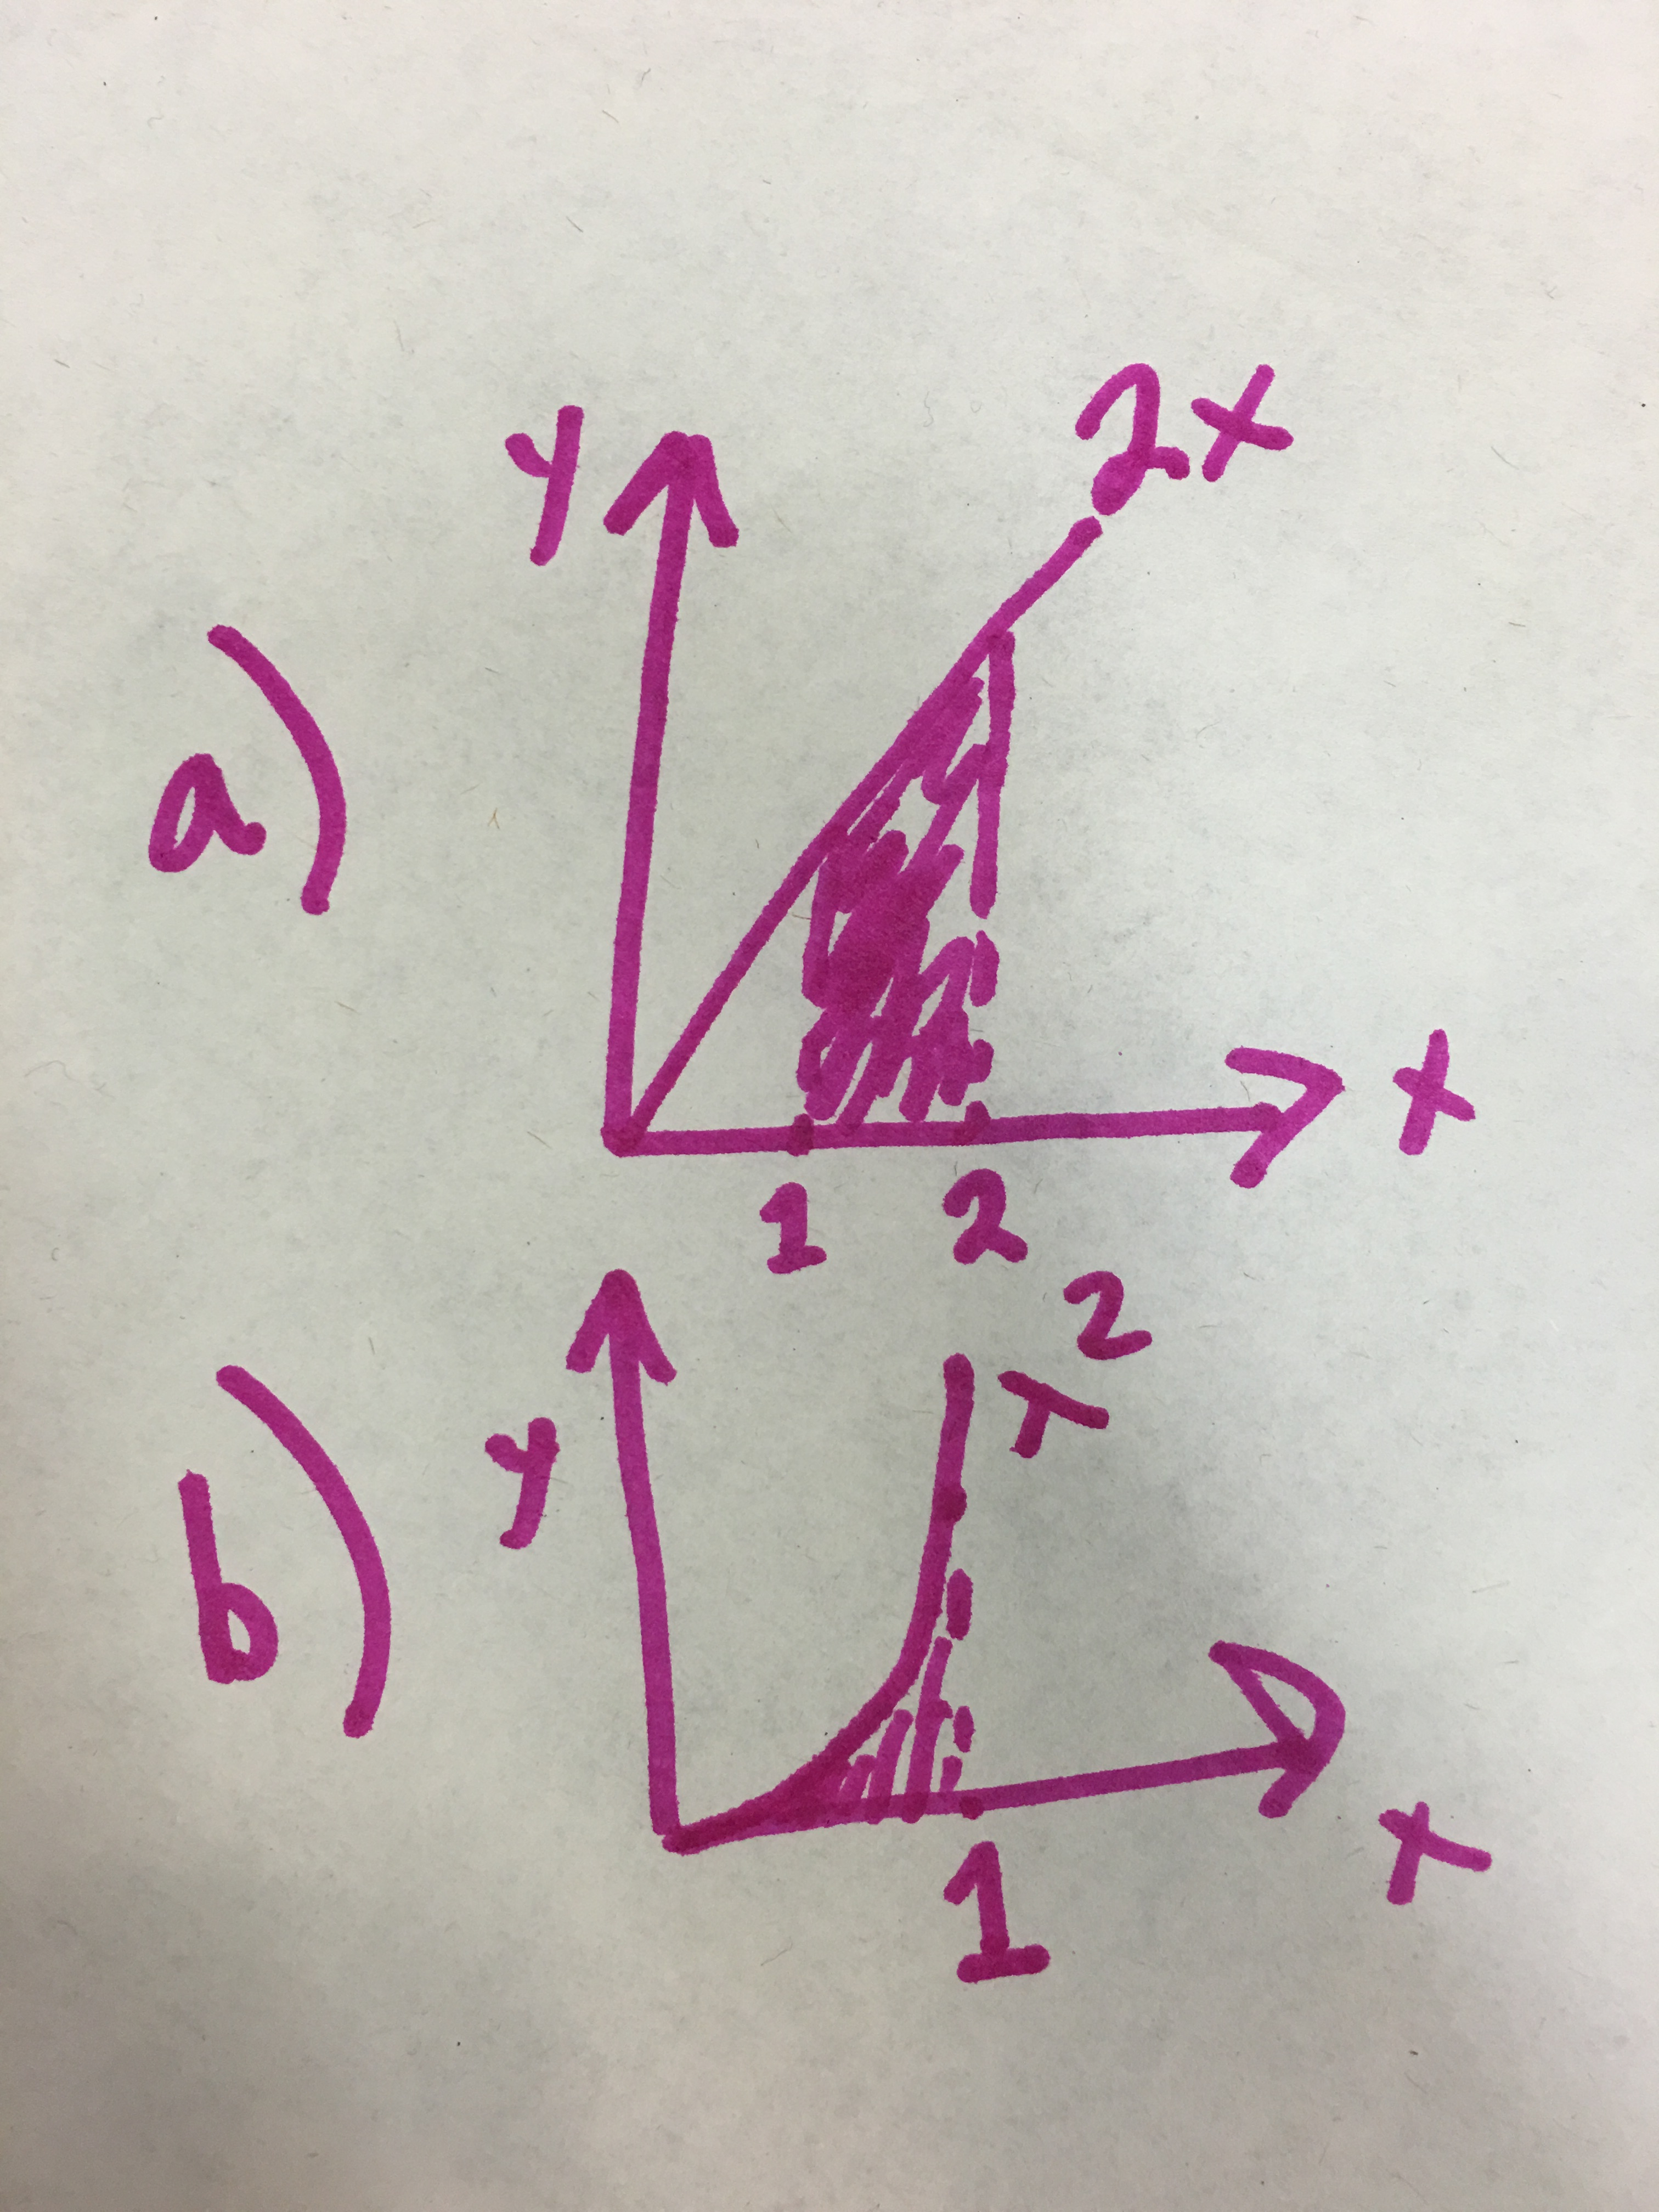
\includegraphics[height=3in]{regions.jpg}
    \caption{The regions of integration.}
\end{figure}

\begin{enumerate}
    \item $\iint\limits_D  \frac{4y}{x^3+2} \; dA, \; D = \{(x,y) | 1 \le x \le 2, 0 \le y \le 2x\} $
    \begin{align*}
        \int_1^2 \int_0^{2x} \frac{4y}{x^3 + 2} dy dx &= \int_1^2 \frac{2y^2}{x^3 + 2}\Bigr|_{0}^{2x} dy dx \\
        &= \int_1^2 \frac{8x^2}{x^3 + 2}dx \\
        u &= x^3 + 2, dx = \frac{du}{3x^2} \\
        \int_1^2 \frac{8x^2}{x^3 + 2}dx  &= \int_3^{10} \frac{8}{3u}du \\
        &= \frac{8}{3} \ln \frac{10}{3}
    \end{align*}
    \item $\iint\limits_D x \cos y \; dA, $ \; D is bounded by $y=0, y = x^2, x = 1$
    \begin{align*}
        \int_0^1 \int_0^{x^2} x \cos y \, dy dx &= \int_0^1 xsiny \Bigr|_{0}^{x^2} dx \\
        &= \int_0^1 x \sin x^2 \, dx \\
        u &= x^2, dx = \frac{du}{2x} \\
        \int_0^1 x \sin x^2 \, dx &= \int_0^1 \frac{1}{2} \sin u \, du \\
        &= -\frac{1}{2}  \cos u \Bigr|_{0}^{1} \\
        &= \frac{1-\cos (1)}{2}
    \end{align*}
\end{enumerate}

\paragraph{18. Visualize the following solids and compute their volume using a double integral.}

\begin{figure}[H]
    \centering
    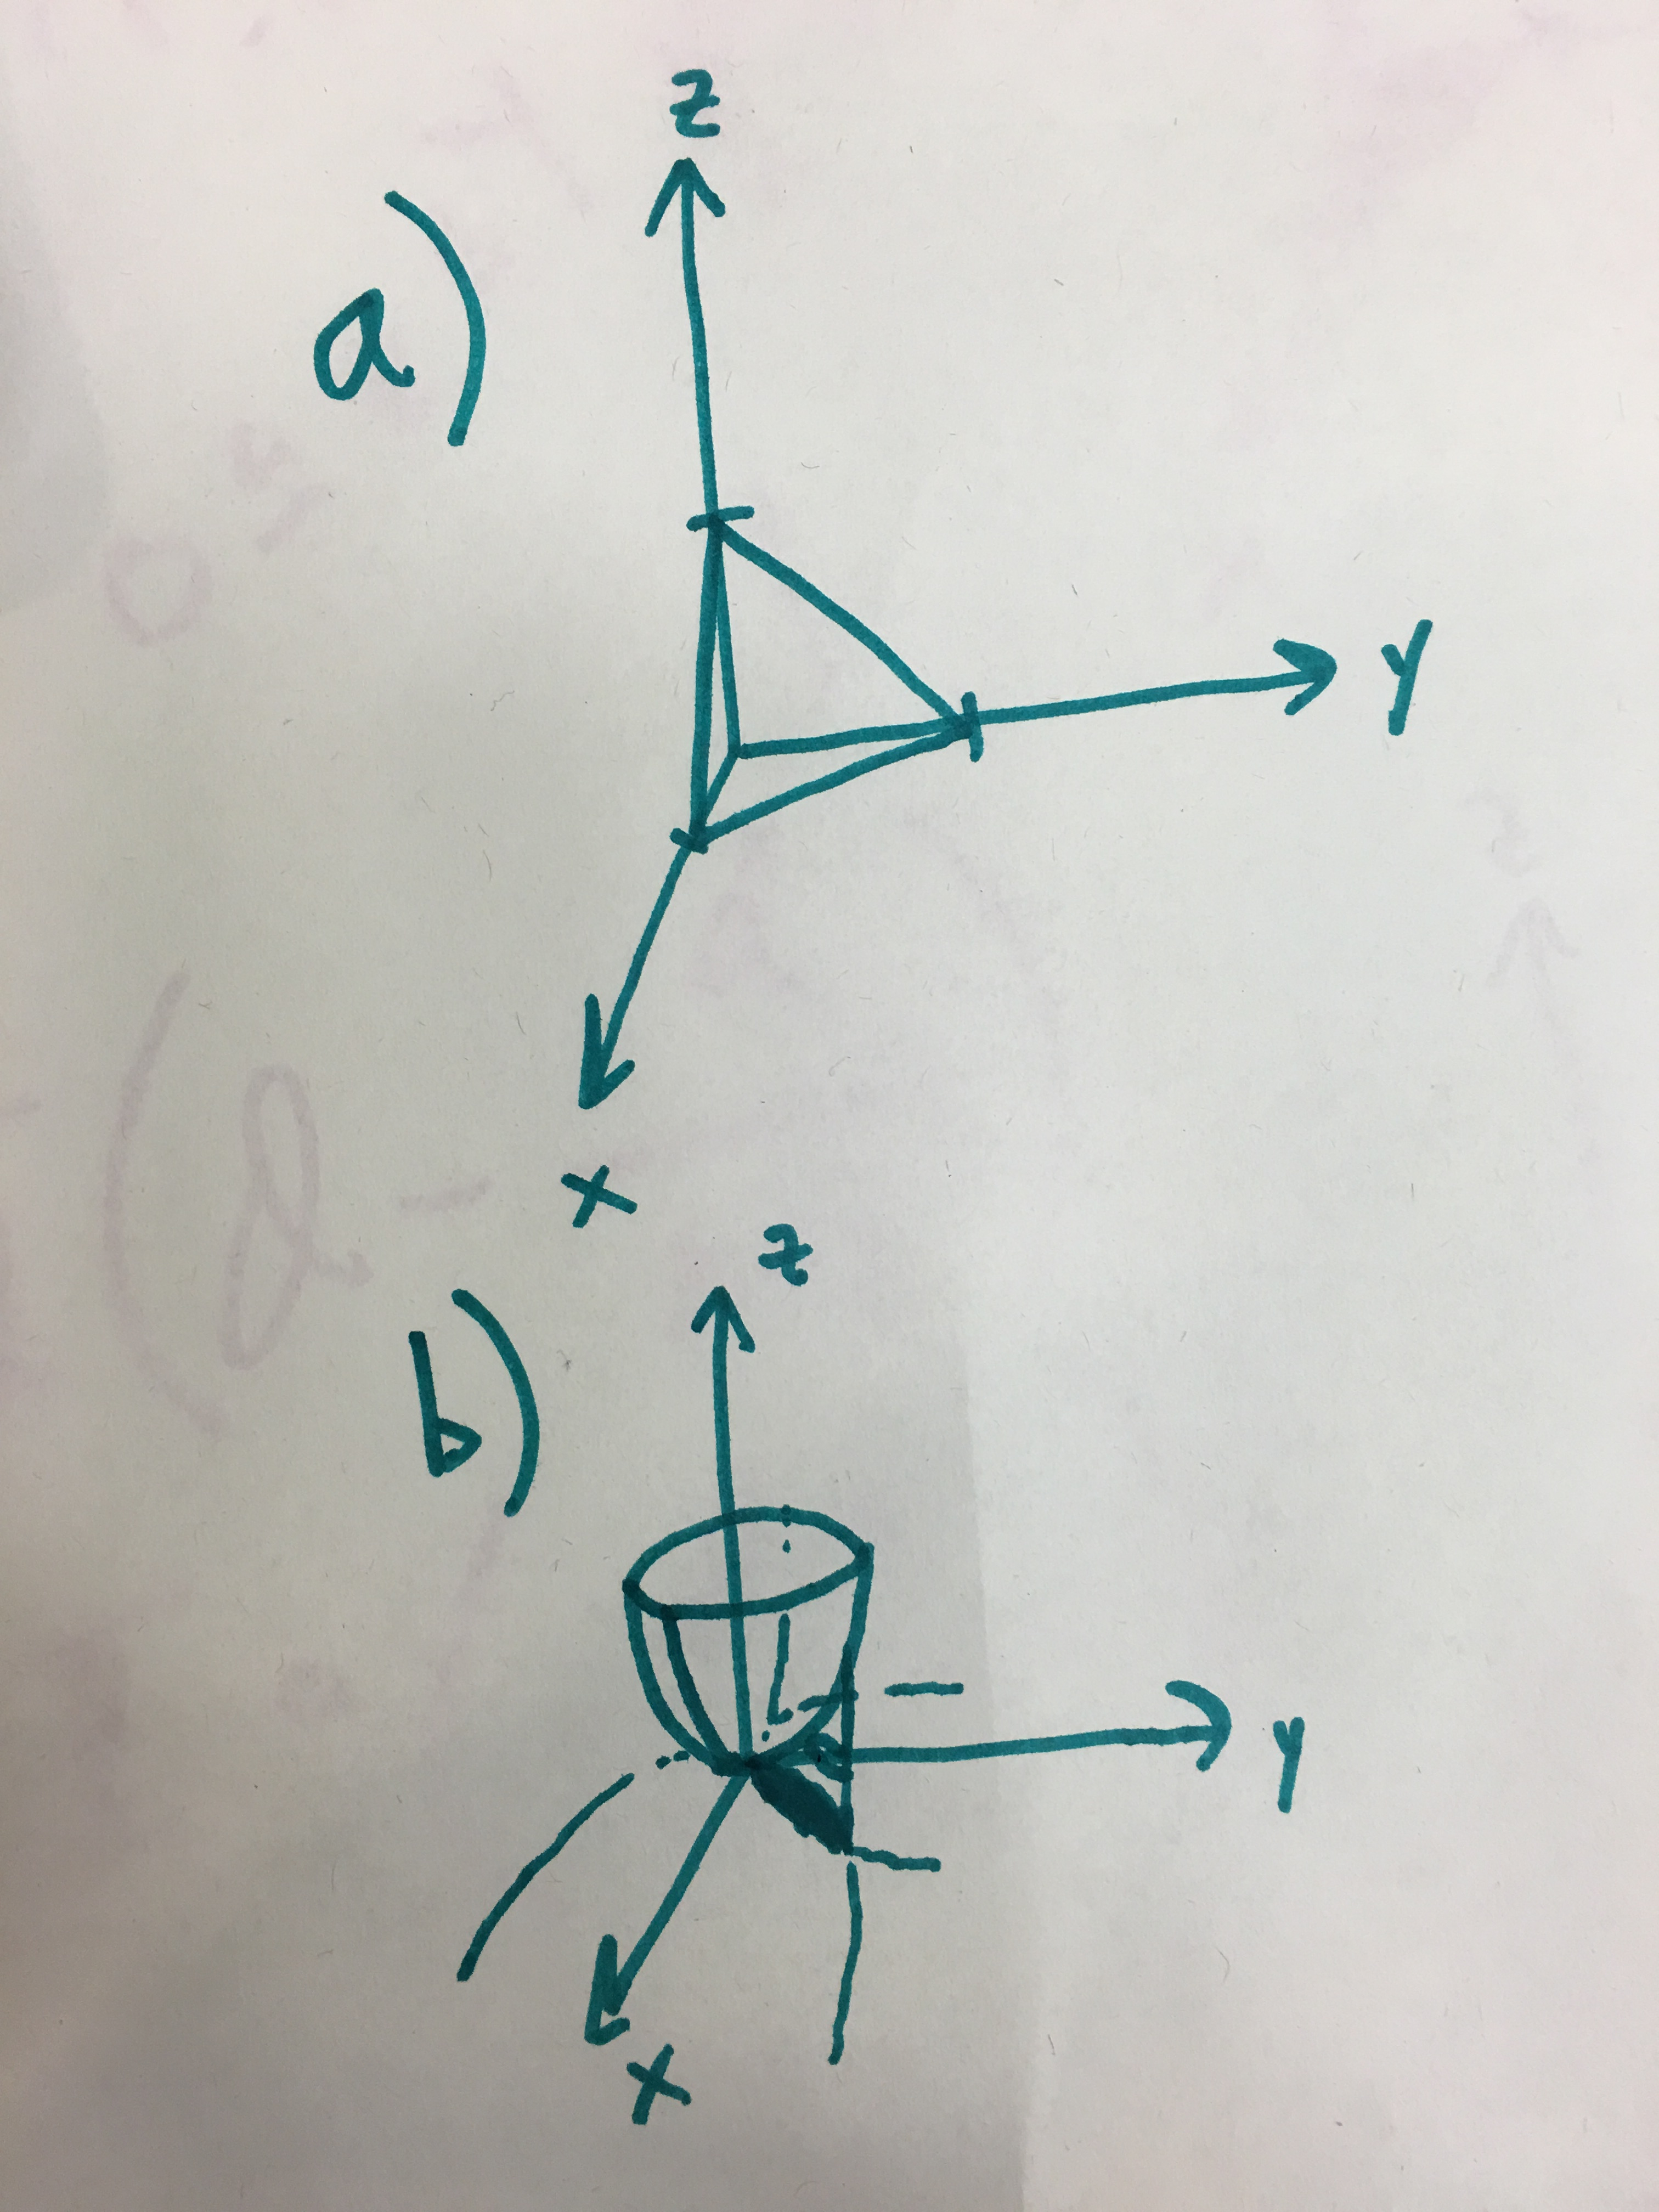
\includegraphics[height=3in]{regions2.jpg}
    \caption{The solids.}
\end{figure}

\begin{enumerate}
    \item Bounded by the planes $x = 0$, $y=0$, $z=0$, and $x+y+z=1$.
    \begin{align*}
        \int_0^1 \int_0^{1-x} (1-x-y) dy dx &= \int_0^1 y(1-x) - \frac{1}{2}y^2 \Bigr|_{0}^{1-x} dx \\
        &= \int_0^1 \left((1-x)^2 - \frac{1}{2}(1-x)^2\right) dx \\
        &= \frac{1}{2} \int_0^1 (x^2 - 2x + 1) dx  \\
        &= \frac{1}{2} \left(\frac{1}{3}x^3 - x^2 + x\right)\Bigr|_{0}^{1} \\
        &= \frac{1}{6}
    \end{align*}
    \item Under the paraboloid $z = x^2 + y^2$ and above the region bounded by $y=x^2$ and $x=y^2$.
    \begin{align*}
        \int_0^1 \int_{x^2}^{\sqrt{x}} \left(x^2 + y^2\right) dy dx &= \int_0^1 yx^2 + \frac{1}{3}y^3 \Bigr|_{x^2}^{\sqrt{x}} dx \\
        &= \int_0^1 \left(x^\frac{5}{2} + \frac{1}{3}x^\frac{3}{2} - x^4 - \frac{1}{3}x^6\right)dx \\
        &= \left(\frac{2}{7}x^\frac{7}{2} + \frac{2}{15}x^\frac{5}{2} - \frac{1}{5}x^5 - \frac{1}{21}x^7\right) \Bigr|_{0}^{1} \\
        &= \frac{6}{35}
    \end{align*}
\end{enumerate}

\paragraph{19. Visualize the solids defined by the limits of integration, and evaluate their volume.}

\begin{figure}[H]
    \centering
    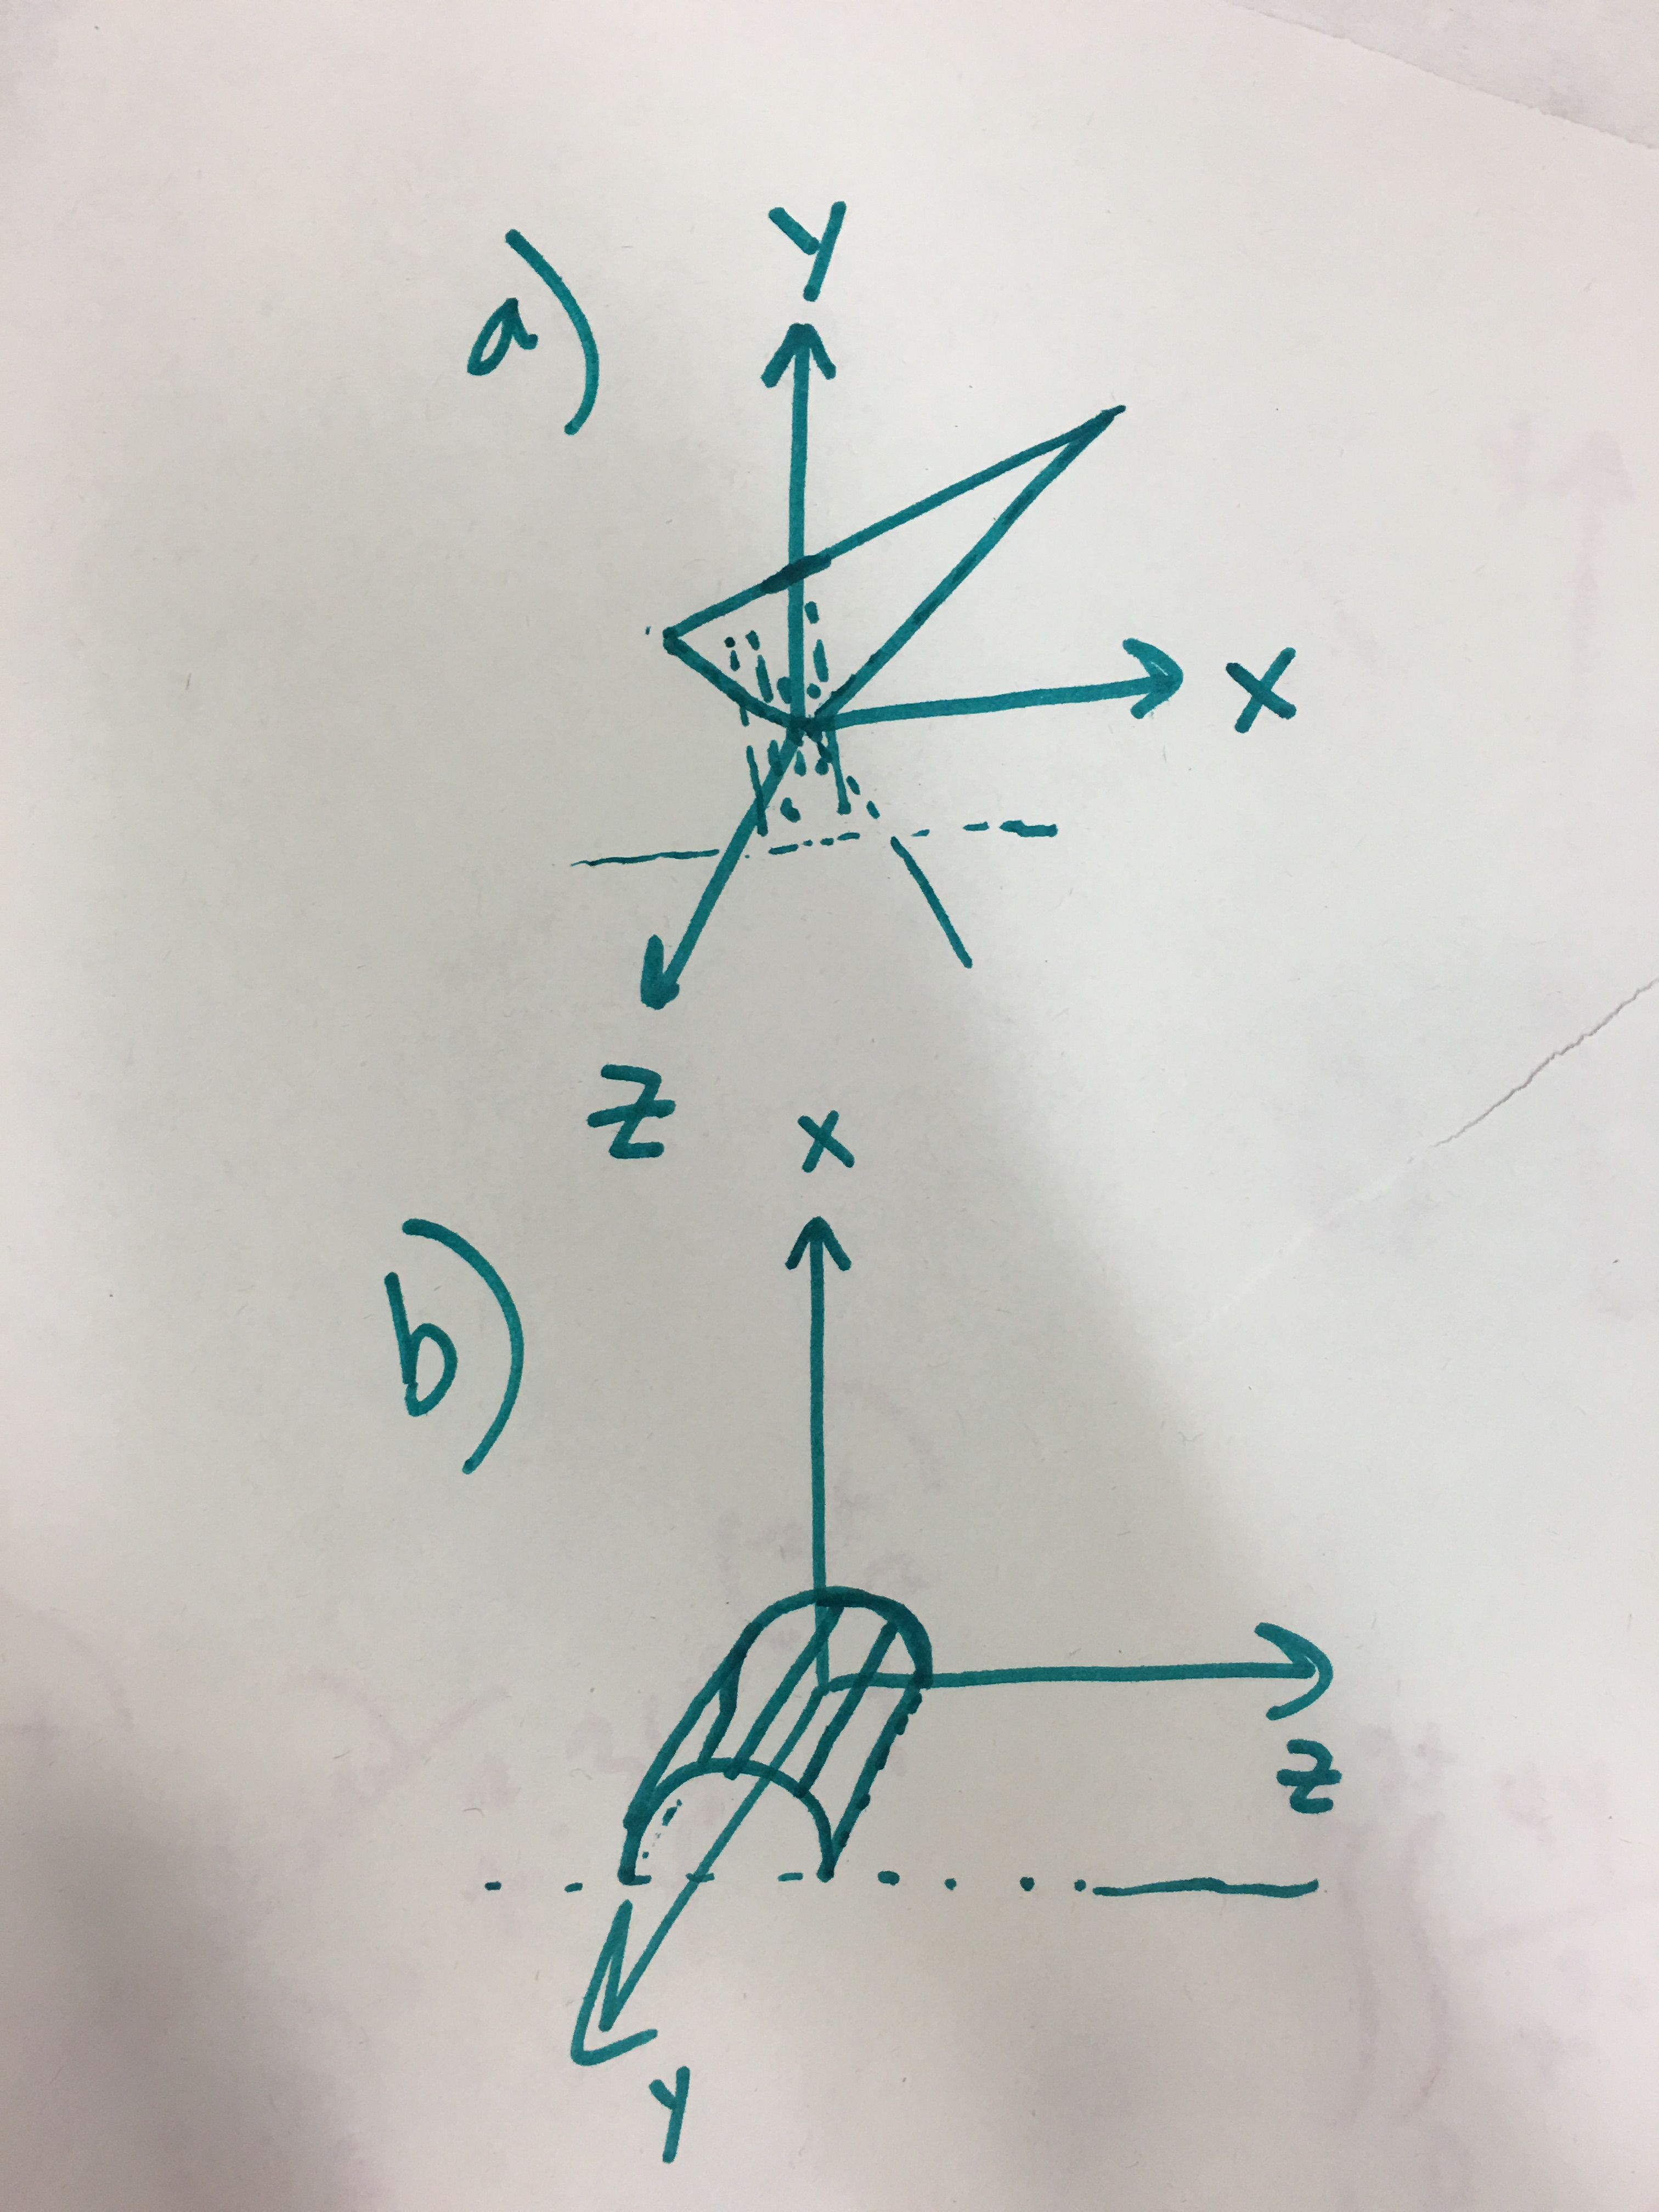
\includegraphics[height=3in]{regions3.jpg}
    \caption{The solids.}
\end{figure}

\begin{enumerate}
    \item $\int_0^1 \int_0^z \int_0^{x+z} \; dy dx dz$
    \begin{align*}
        &= \int_0^1 \int_0^z (x + z) \, dxdz  \\
        &= \int_0^1 \frac{1}{2}x^2 + zx \Bigr|_{0}^{z} dz \\
        &= \int_0^1 \left(\frac{1}{2}z^2 + z^2\right) \, dz \\
        &= \frac{1}{2} z^3 \Bigr|_{0}^{1} \\
        &= \frac{1}{2}
    \end{align*}
    \item $\int_0^3 \int_0^1 \int_0^{\sqrt{1-z^2}} \; dx dz dy$
    \begin{align*}
        \int_0^3 \int_0^1 \int_0^{\sqrt{1-z^2}} \, dx dz dy &= \int_0^3 \int_0^1 \sqrt{1-z^2} \, dz dy \\
        &= \int_0^3 \frac{1}{2}\left(z\sqrt{1-z^2} + \sin^{-1} z\right)\Bigr|_{0}^{1} dy \\
        &= \frac{1}{2} \int_0^3 \frac{\pi}{2}dy \\
        &= \frac{3\pi}{4}
    \end{align*}
\end{enumerate}

\paragraph{20. Visualize the solid defined by the limits of integration, and figure out the five other triple integrals that are the same.}

\begin{enumerate}
    \item $\int_0^1 \int_y^1 \int_0^y \; dz dx dy$
    \newline Below is the visualization of the volume bounded by the integral
    \begin{figure}[H]
        \centering
        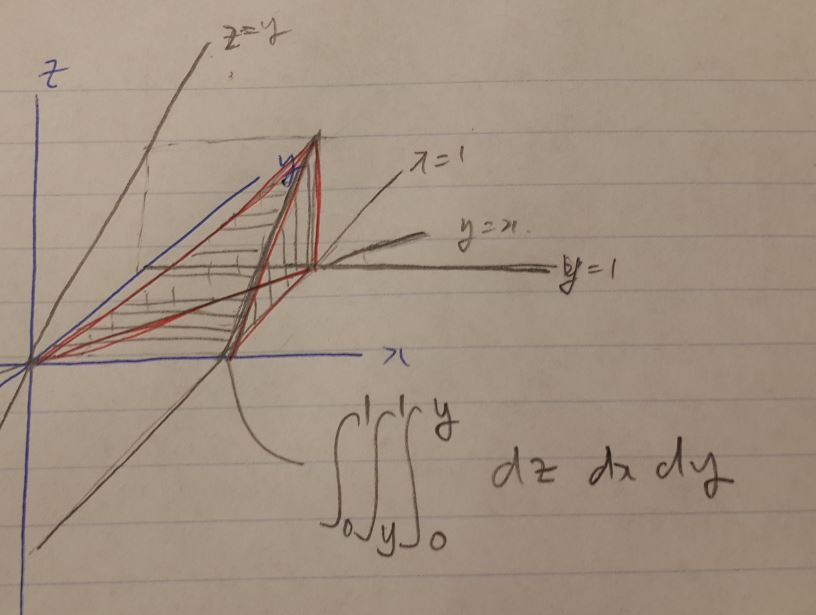
\includegraphics[width=0.75\columnwidth]{num201.JPG}
        \caption{Volume bounded by the integral}
        \label{fig:my_label}
    \end{figure}
    \newline Here are the five equivalent integrals:
    \begin{enumerate}
        \item $\int_0^1 \int_0^x \int_0^y \; dz dy dx$ 
        \item $\int_0^1 \int_z^1 \int_y^1 \; dx dy dz$
        \item $\int_0^1 \int_0^z \int_0^x \; dy dx dz$
        \item $\int_0^1 \int_0^y \int_y^1 \; dx dz dy$
        \item $\int_0^1 \int_0^x \int_0^x \; dy dz dx$
    \end{enumerate}
    \item $\int_0^1 \int_0^{1-x^2} \int_0^{1-x} \; dy dz dx$
    \newline Below is the visualization of the volume bounded by the integral
    \begin{figure}[H]
        \centering
        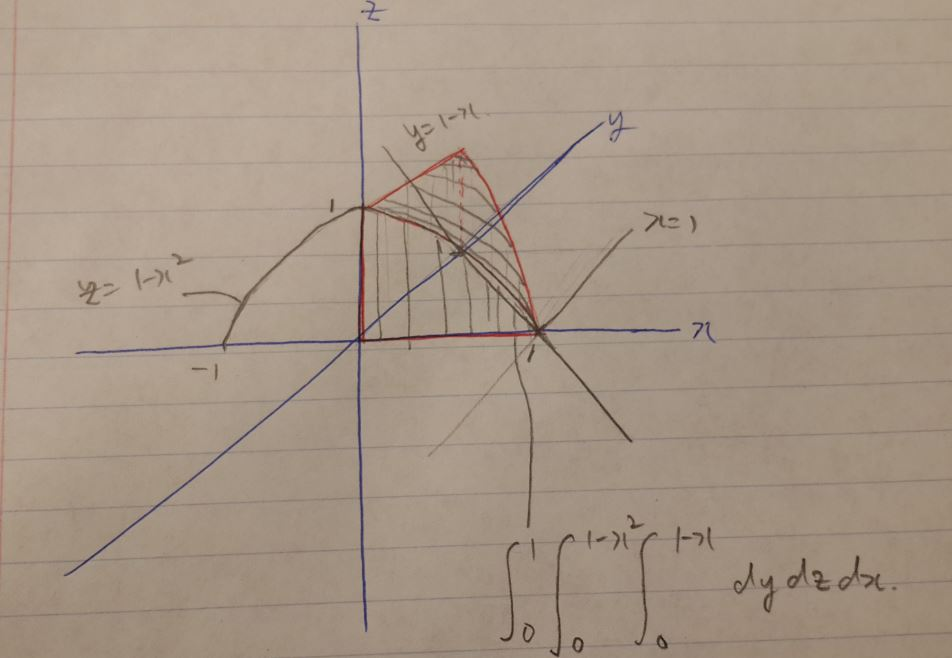
\includegraphics[width=0.75\columnwidth]{num20_2.JPG}
        \caption{Volume bounded by the integral}
        \label{fig:my_label}
    \end{figure}
    \newline Here are the five equivalent integrals:
    \begin{enumerate}
        \item $\int_0^1 \int_0^{\sqrt{1-z}} \int_0^{1-x} \; dy dx dz$
        \item $\int_0^1 \int_0^{1-x} \int_0^{1-x^2} \; dz dy dx$
        \item $\int_0^1 \int_0^{1-y} \int_0^{1-x&2} \; dz dx dy$
        \item $\int_0^1 \int_0^{1-x} \int_0^{\sqrt{1-z}} \; dx dy dz$
        \item $\int_0^1 \int_0^{1-x^2} \int_0^{1-y} \; dx dz dy$ 
    \end{enumerate}
    \newline However, (d) and (e) are not allowed since their limits of integration include a variable that is integrated beforehands.
    
    \newline You can think of them as a piece wise function where from 0 to y in z axis, the surface function is 1-x, and from y to 1 in z axis, the surface function is 1-$x^2$.
    
    \newline So (d) and (e) becomes:
    \begin{enumerate}
        \item $\int_0^1 \int_z^{1} \int_0^{1-y} \; dx dy dz + \int_0^1 \int_0^{z} \int_0^{\sqrt{1-z}} \; dx dy dz$
        \item $\int_0^1 \int_y^{1} \int_0^{\sqrt{1-z}} \; dx dz dy + \int_0^1 \int_0^{y} \int_0^{1-y} \; dx dz dy$
    \end{enumerate}
    
\end{enumerate}

\paragraph{21. Visualize the solids defined by the limits of integration, and evaluate the triple integrals.}
    \begin{enumerate}
        \item $\int_0^1 \int_x^{2x} \int_0^y 2xyz \; dz dy dx$
        \newline Here is the region bounded by the integration ranges.
        
        
        \begin{figure}[H]
            \centering
            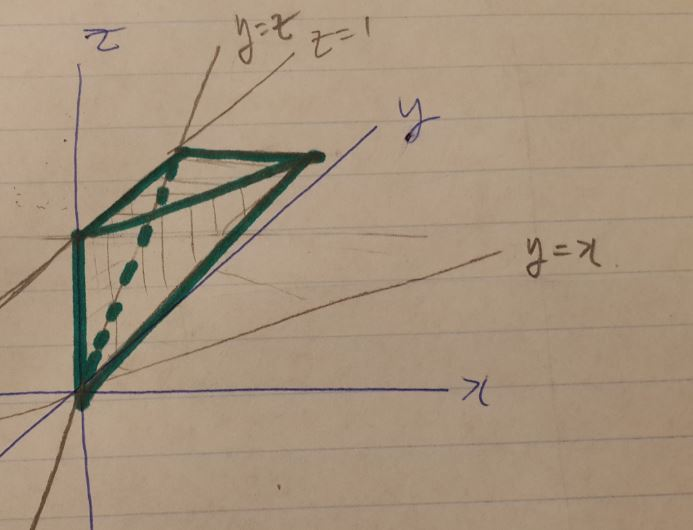
\includegraphics[width=0.75\columnwidth]{num21_1.JPG}
            \caption{Region bounded by the integration ranges}
            \label{fig:my_label}
        \end{figure}
\begin{align*}
    \int_0^1 \int_x^{2x} \int_0^y 2xyz \; dz dy dx &= \int_0^1 \int_x^{2x} xyz^2 \Bigr|_{0}^{y} \; dy dx \\
    &= \int_0^1 \int_x^{2x} xy^3 \; dy dx \\
    &= \int_0^1 x\frac{1}{4}y^4 \Bigr|_{x}^{2x} \; dx \\
    &= \int_0^1 \frac{1}{4}x(16x^4-x^4) \; dx\\
    &= \int_0^1 \frac{15}{4}x^5 \; dx\\
    &= \frac{15}{24}x^6 \Bigr|_{0}^{1}\\
    &= \frac{5}{8}
\end{align*}
        
        
        \item $\int_0^1 \int_0^z \int_0^y z e^{-y^2} \; dx dy dz$
        \newline Here is the region bounded by the integration ranges.
        
        \begin{figure}[H]
            \centering
            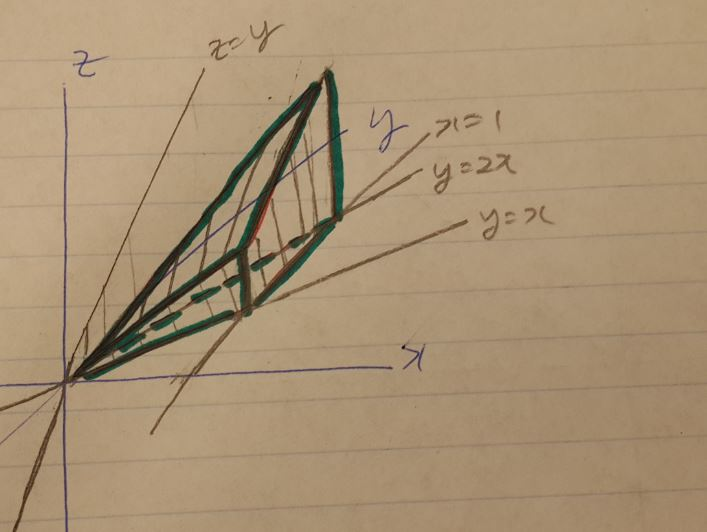
\includegraphics[width=0.75\columnwidth]{num21_2.JPG}
            \caption{Region bounded by the integration ranges}
            \label{fig:my_label}
        \end{figure}
        
\begin{align*}
    \int_0^1 \int_0^z \int_0^y z e^{-y^2} \; dx dy dz &= \int_0^1 \int_0^z z e^{-y^2}x\Bigr|_{0}^{y} \; dy dz \\
    &=\int_0^1 \int_0^z zy e^{-y^2}\; dy dz\\
    &=\int_0^1 z \frac{-1}{2}e^{-y^2}\Bigr|_{0}^{z}\; dz\\
    &=\int_0^1 \frac{-1}{2}ze^{-z^2}\; dz \\
    &= \frac{1}{4}e^{-z^2}\Bigr|_{0}^{1}\\
    &= \frac{1}{4e}-\frac{1}{4}
\end{align*}
    \end{enumerate}

\paragraph{22. Find the total mass of the following plates and solids.}

\begin{enumerate}
    \item The plate bounded by the parabola $y = 9 - x^2$ and the x-axis; mass (or charge) density $\rho(x,y) = y$.

        \newline Here is the region bounded by the integration ranges.
        
        
        \begin{figure}[H]
            \centering
            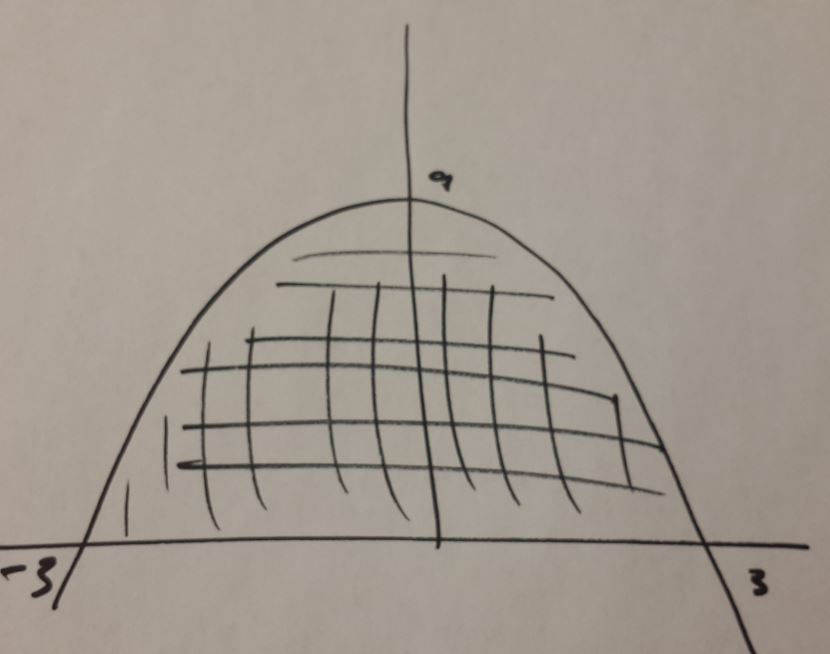
\includegraphics[width=0.75\columnwidth]{num22_1.JPG}
            \caption{Region bounded by the integration ranges}
            \label{fig:my_label}
        \end{figure}
\begin{align*}
    \int_{-3}^3 \int_0^{9-x^2} y \; dy dx 
    &= \int_{-3}^3 0.5y^2 \Bigr|_{0}^{9-x^2} \; dx \\
    &= \int_{-3}^3 81 - 18x^2 + x^4 \; dx \\
    &= 81x - 6x^3 + \frac{1}{5}x^5 \Bigr|_{-3}^{3}\\
    &= 129.6 
\end{align*}
        
    
    \item The tetrahedron bounded by the planes $x=0$, $y=0$, $z=0$, and $x+y+z=1$; mass density $\rho(x,y,z) = y$.
            \newline Here is the region bounded by the integration ranges.
        
        \begin{figure}[H]
            \centering
            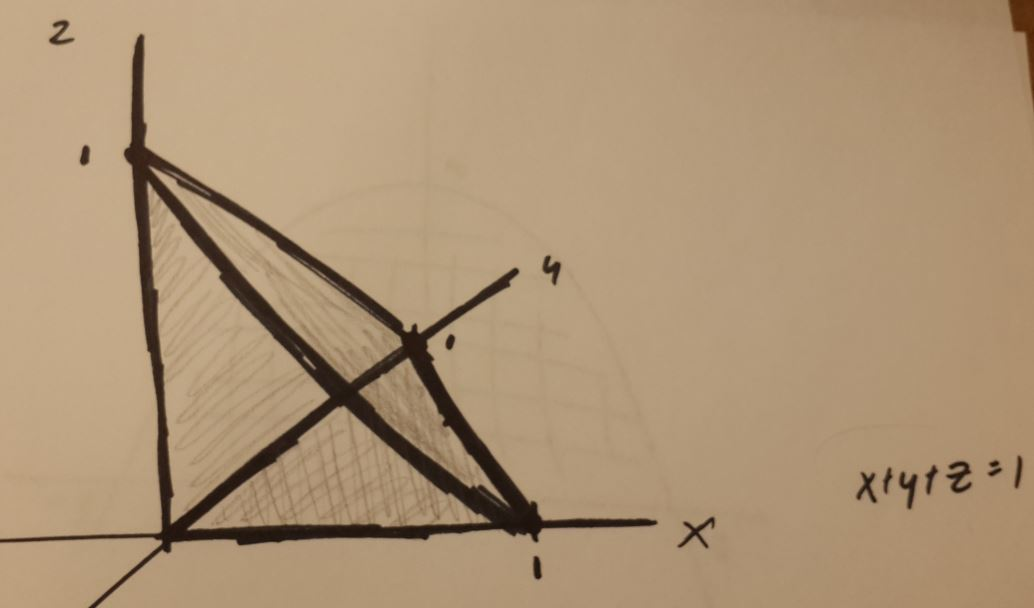
\includegraphics[width=0.75\columnwidth]{num22_2.JPG}
            \caption{Region bounded by the integration ranges}
            \label{fig:my_label}
        \end{figure}
        
\begin{align*}
    \int_0^1 \int_0^{1-x} \int_0^{1-x-y} y\; dz dy dx \\
    &= \frac{1}{24}
\end{align*}
    \end{enumerate}
\end{enumerate}

\end{document}
